%!TeX root=../tese.tex
%("dica" para o editor de texto: este arquivo é parte de um documento maior)
% para saber mais: https://tex.stackexchange.com/q/78101

\chapter{Implementação da simulação} 
\label{cap_mvp}

O MVP da ferramenta de simulações interativas de conceitos de lógica de programação está disponível no link: \url{https://mariliatd.github.io/logic-sims-mvp/}. A tela inicial da simulação \enquote{Planejando a Festa} pode ser observada na Figura \ref{figure:tela_inicial}. Ela apresenta uma barra de navegação no topo da página, com o nome da simulação e um link de \enquote{ajuda}, o qual abre um diálogo contendo descrições do conceitos de programação abordados. Abaixo dela, há o espaço da simulação que, inicialmente, apresenta um quadro com informações sobre a ferramenta, e o espaço do pseudocódigo à direita.

\begin{figure}[h!]
    \centering
    \setlength{\fboxrule}{0.1pt} % espessura da borda da figura
    \fbox{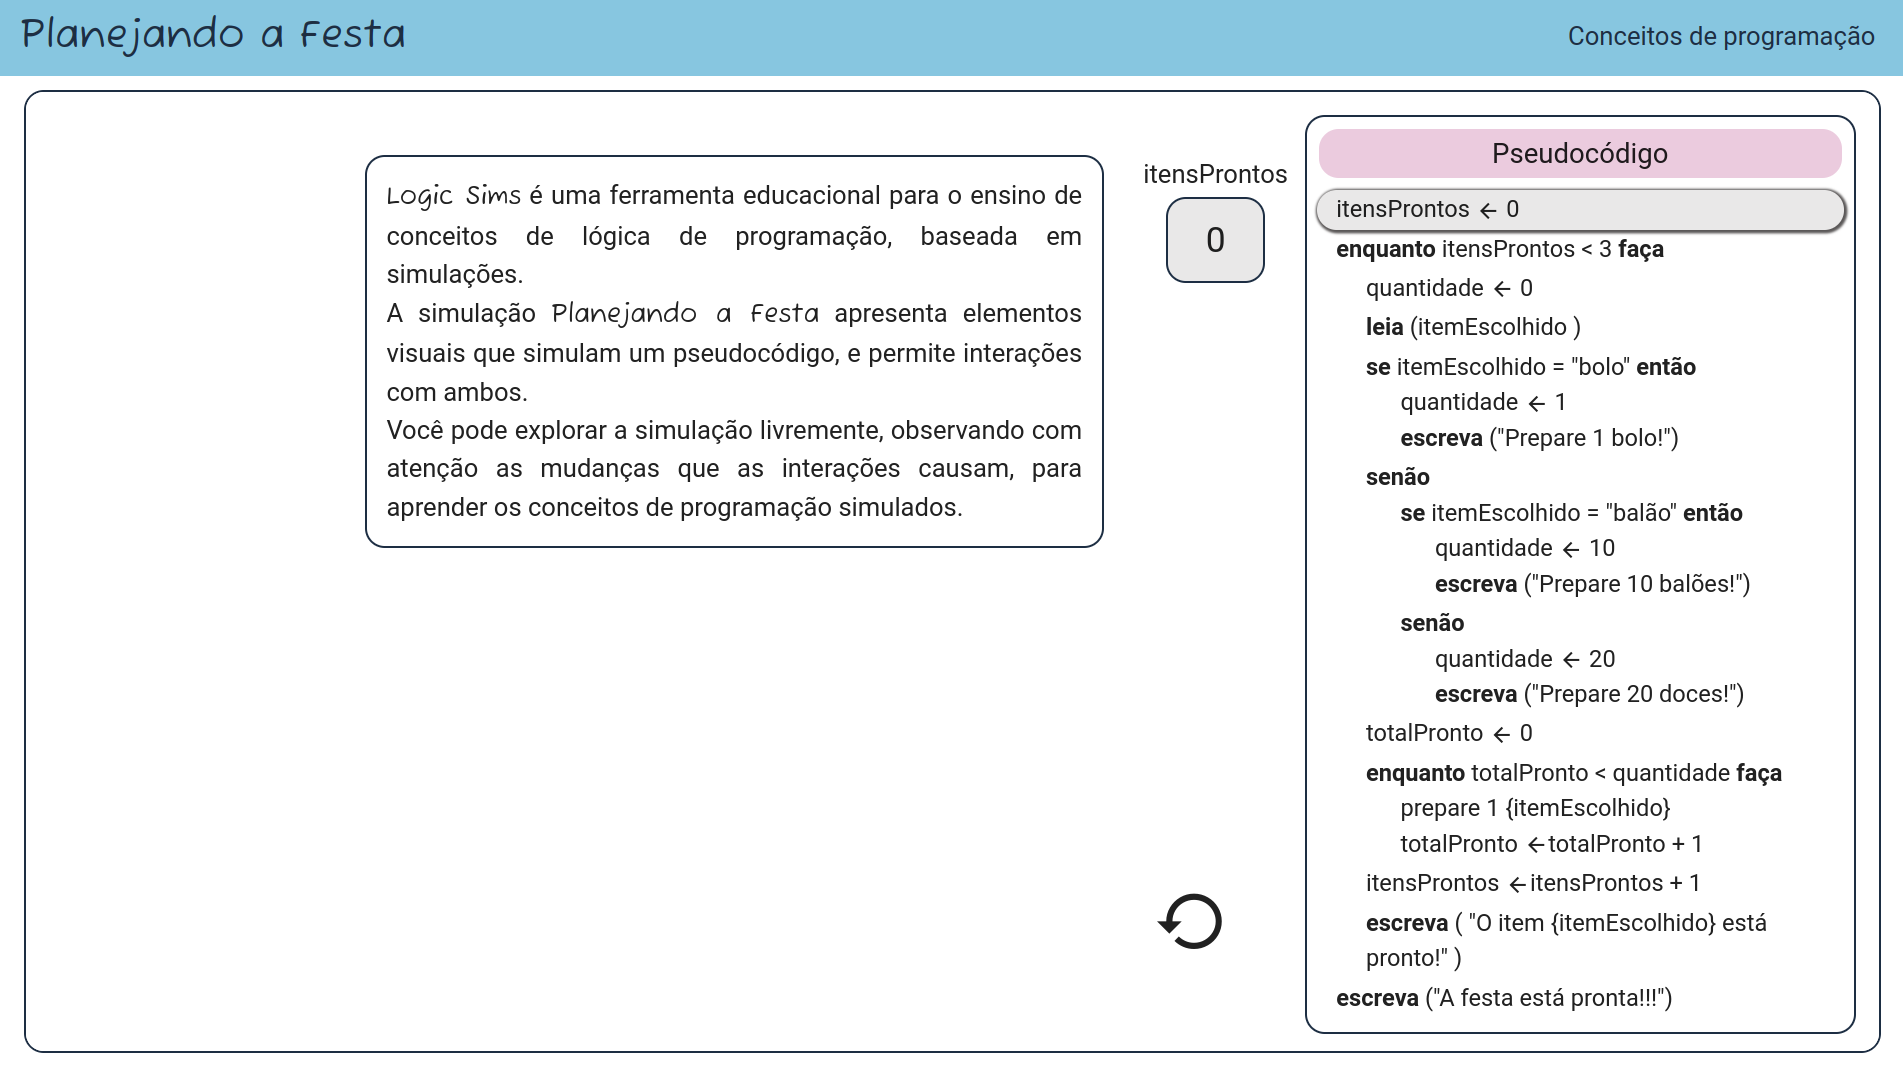
\includegraphics[scale=0.22]{tela_inicial_mvp.png}}
    \caption{Tela inicial do MVP da simulação \enquote{Planejando a Festa}.}
    \label{figure:tela_inicial}
\end{figure}

Nessa tela, é possível visualizar algumas das alterações sugeridas na etapa de validação dos protótipos. Essa nova versão da simulação também permite interações com o pseudocódigo, o qual tem as linhas destacadas com uma borda com uma animação que pisca quando é necessário interagir com ela. Esse recurso foi implementado para facilitar a visualização da \enquote{execução} de cada passo do pseudocódigo, o qual foi modificado. Adicionamos à lógica da simulação um laço de repetição externo para realizar a iteração na preparação dos três itens disponíveis para compor a festa, que faltava no projeto do protótipo.

Assim, a simulação permite selecionar três itens em quantidades distintas e preparar cada um até atingir as quantidades correspondentes até que a festa esteja pronta. A seleção de um item pelo usuário representa a entrada ou leitura de um valor no pseudocódigo, que condiciona a quantidade de itens a serem preparados. Ao escolher um item ou finalizar o seu preparo e quando a festa está pronta são impressas mensagens na tela em uma janela representando a saída de dados no pseudocódigo, como mostra a Figura \ref{figure:saida}. 

\begin{figure}[h!]
    \centering
    \setlength{\fboxrule}{0.1pt} % espessura da borda da figura
    \fbox{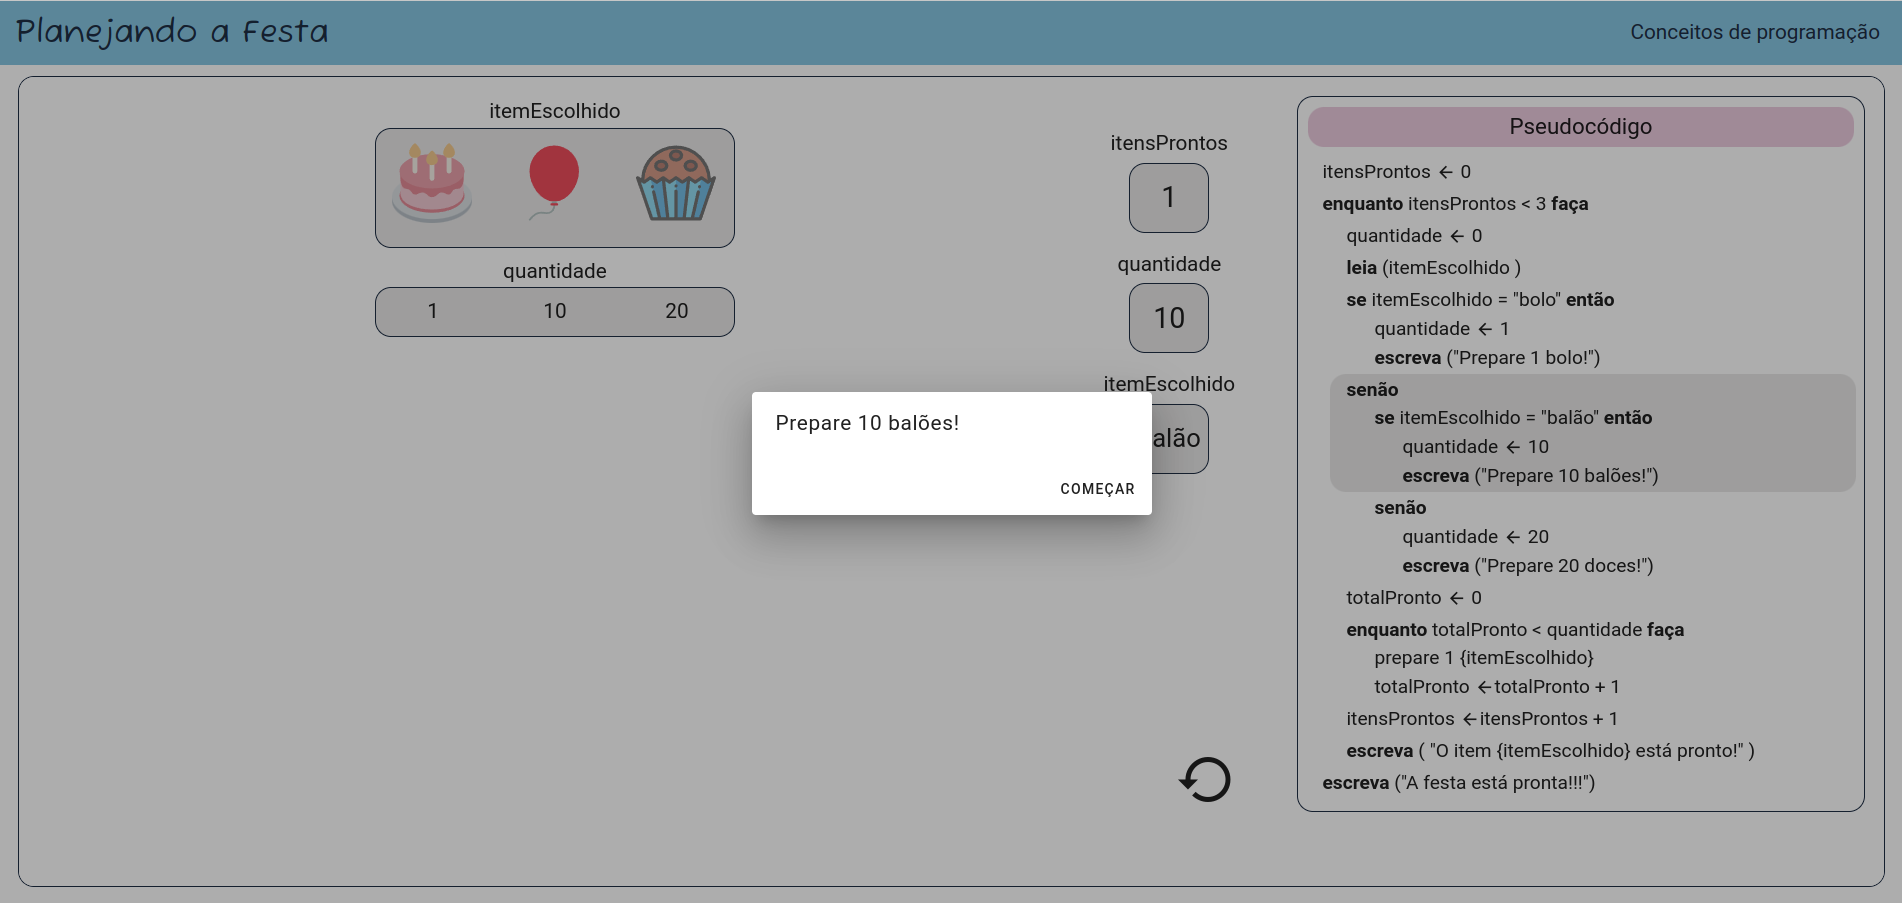
\includegraphics[scale=0.22]{saida.png}}
    \caption{Representação visual do conceito de saída com a mensagem \enquote{impressa} na tela.}
    \label{figure:saida}
\end{figure}

Quando o usuário seleciona um item para preparo, a escolha dos demais fica desabilitada, para que a interação com a simulação siga o fluxo do pseudocódigo e não permita que o usuário troque de item enquanto está dentro do laço de repetição interno, por exemplo. A Figura \ref{figure:item_escolhido} mostra o cenário em que o item \enquote{bolo} foi selecionado e os demais estão sombreados, não sendo possível clicar neles. Ainda, após o preparo de um item, este fica desabilitado para escolha na iteração seguinte, limitando o preparo dos três itens (em qualquer ordem) para finalizar o preparo da festa e a simulação.

\begin{figure}[h!]
    \centering
    \setlength{\fboxrule}{0.1pt} % espessura da borda da figura
    \fbox{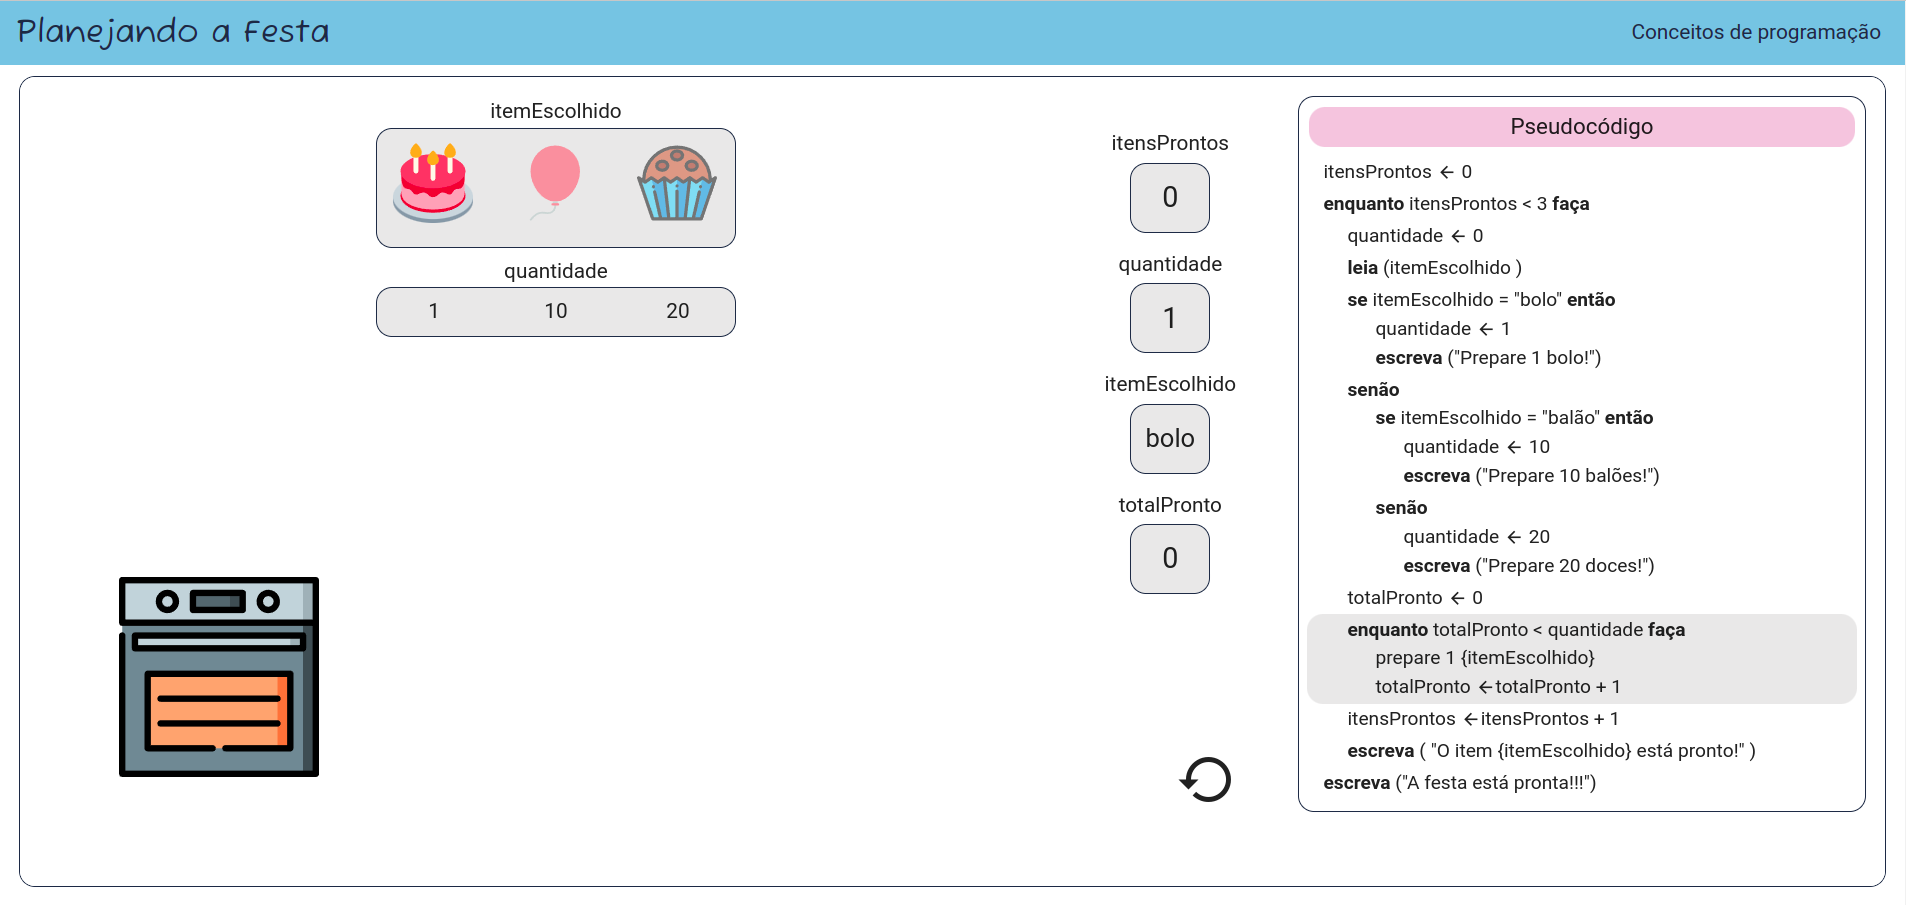
\includegraphics[scale=0.22]{item_escolhido.png}}
    \caption{Escolhendo um item na simulação \enquote{Planejando a Festa}.}
    \label{figure:item_escolhido}
\end{figure}

Na Figura \ref{figure:item_escolhido} também podemos observar que cada variável está separada em um elemento visual próprio. Além disso, removemos o controle do incremento do contador que indica a quantidade total pronta de cada item, deixando essa interação apenas nas figuras de preparo de cada item (fogão, cilindro de gás e pratos) para representar o laço de repetição interno do pseudocódigo. Ainda, adicionamos o pseudocódigo para a execução das atividades de preparo do item escolhido dentro desse laço.

Outro recurso incorporado no pseudocódigo da simulação foi a adição de cores para diferenciar os conceitos de lógica de programação, o qual é comumente utilizado nas linguagens de programação em blocos. A escolha das cores foi feita através da ferramenta Coolors\footnote{\url{coolors.co}} que além de apresentar um gerador de paleta de cores, também disponibiliza um verificador de contraste. Ela segue as Diretrizes de Acessibilidade para Conteúdo \textit{Web} (\textit{Web Content Accessibility Guidelines - WCAG}), a qual define uma série de recomendações para tornar a web mais acessível \citep{caldwell2008web}. A categorização das cores foi feita da seguinte forma:

\definecolor{variables}{HTML}{F9F1A8}
\definecolor{inputOutput}{HTML}{FFC17C}
\definecolor{operators}{HTML}{D0F4DE}
\definecolor{conditional}{HTML}{E4C1F9}
\definecolor{loop}{HTML}{A9DEF9}

\begin{itemize}
    \item \colorbox{variables}{Variáveis} (amarelo)
    \item \colorbox{inputOutput}{Entrada} e \colorbox{inputOutput}{saída} (laranja)
    \item \colorbox{operators}{Operadores} (verde)
    \item \colorbox{conditional}{Condicionais} (roxo)
    \item \colorbox{loop}{Laço de repetição} (azul)
\end{itemize}

\noindent Além disso, a simulação mostra o nome de cada conceito de lógica de programação. Esse recurso pode ser visualizado ao passar o mouse em cima de cada conceito. A Figura \ref{figure:pseudocodigo_destaque} apresenta as alterações destacadas.

\begin{figure}[h!]
    \centering
    \setlength{\fboxrule}{0.1pt} % espessura da borda da figura
    \fbox{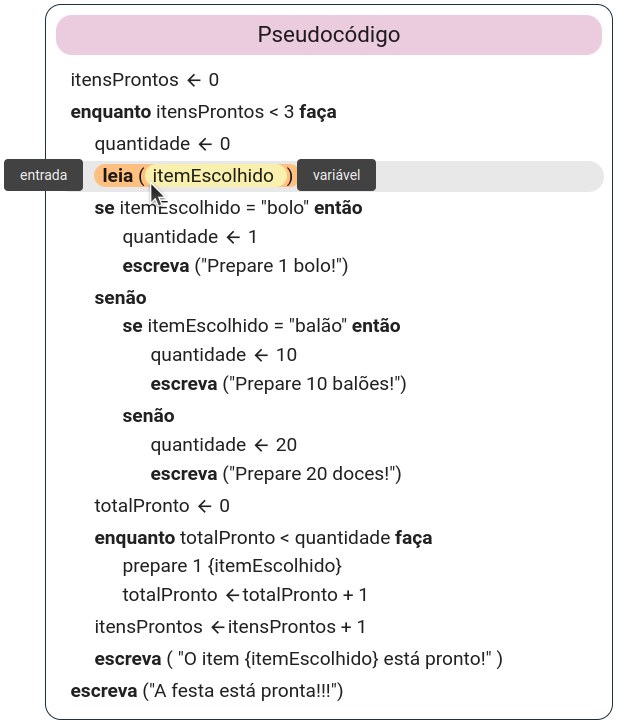
\includegraphics[scale=0.32]{pseudocodigo_destaque1.png}
    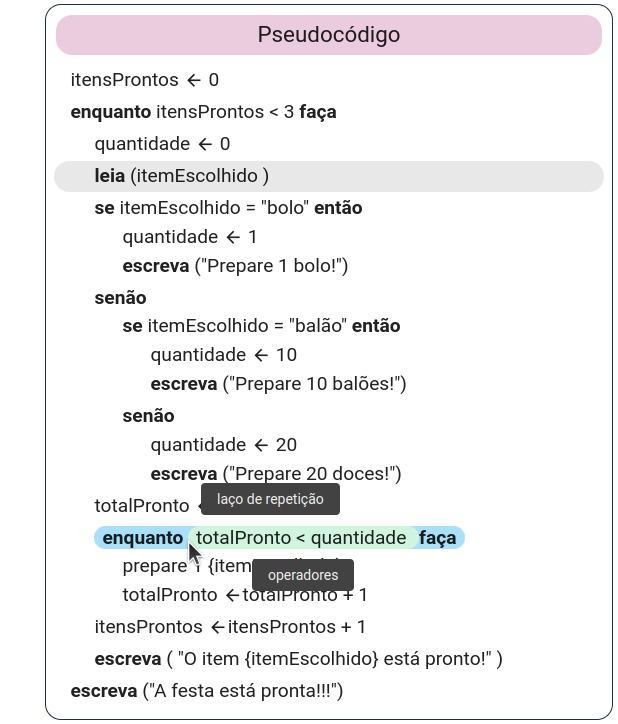
\includegraphics[scale=0.35]{pseudocodigo_destaque2.png}}
    \caption{Destaques do pseudocódigo da simulação \enquote{Planejando a Festa} mostrando a separação em cores por conceito de lógica de programação e a indicação do nome deles ao passar o mouse por cima de cada um.}
    \label{figure:pseudocodigo_destaque}
\end{figure}

Por fim, o \textit{link} para \enquote{Ajuda} na barra de navegação foi renomeado para \enquote{Conceitos de programação} e ele abre uma caixa de diálogo contendo definições de cada conceito, com figuras e exemplos (Figura \ref{figure:conceitos_programacao}). As definições contêm pseudocódigos de exemplo que seguem o esquema de cores descrito acima.

\begin{figure}[h!]
    \centering
    \setlength{\fboxrule}{0.1pt} % espessura da borda da figura
    \fbox{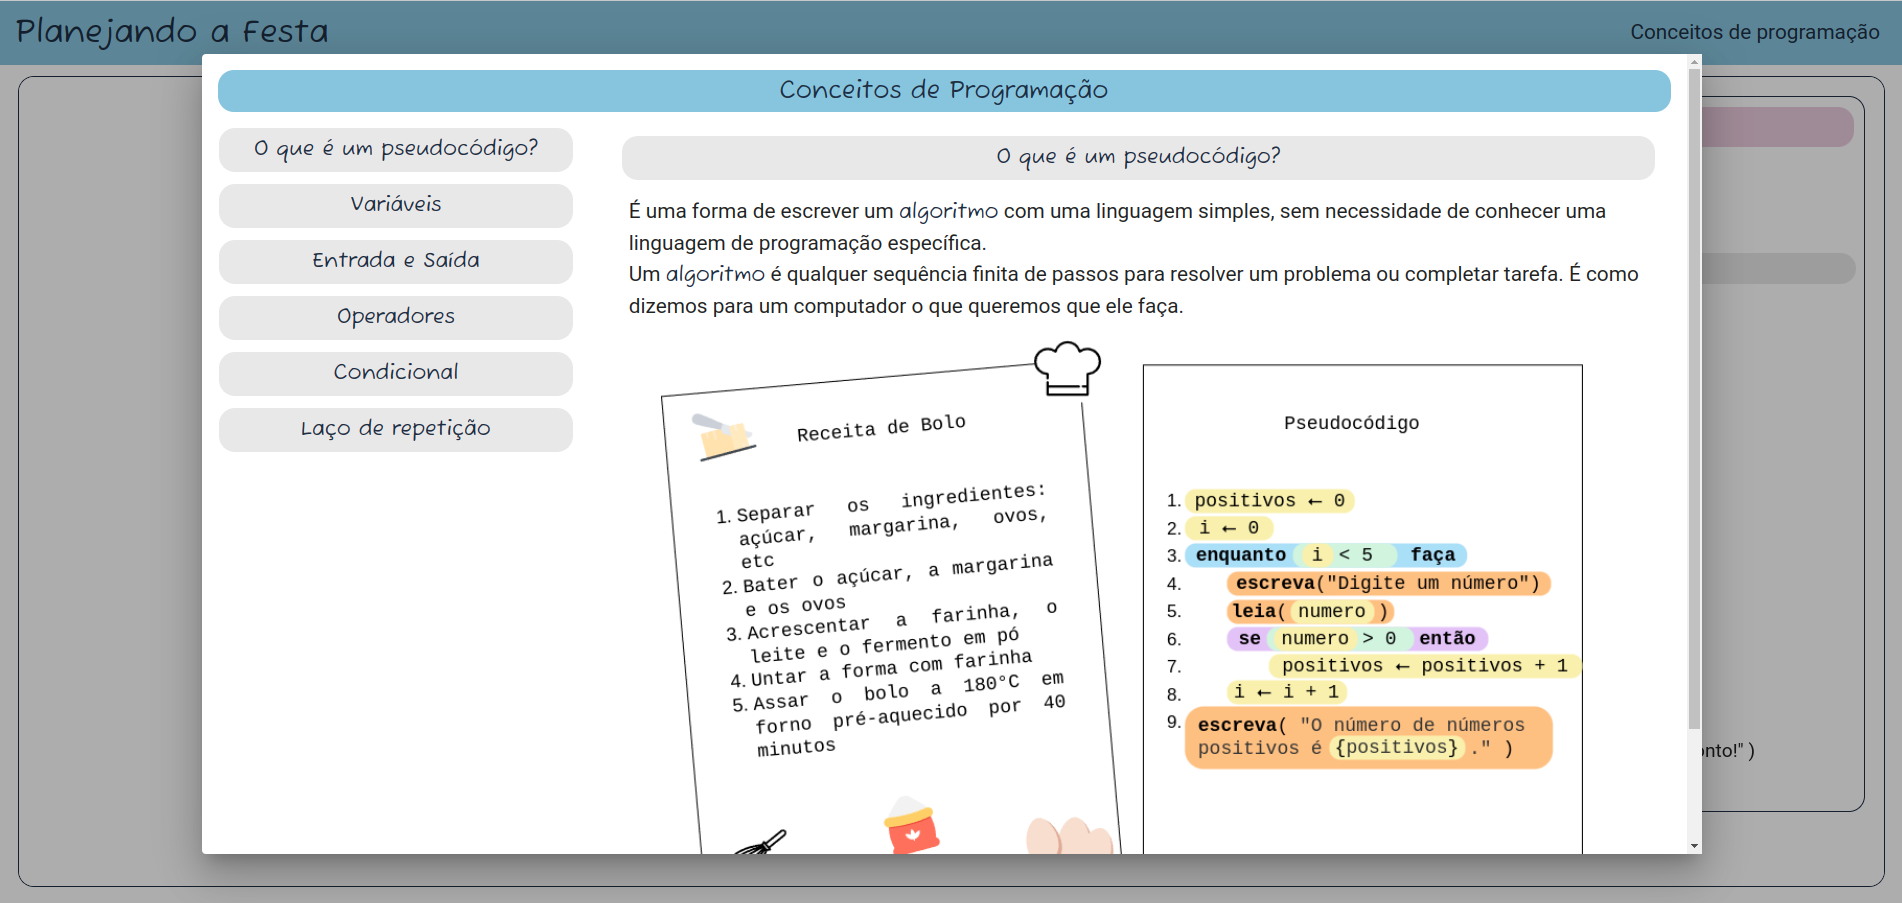
\includegraphics[scale=0.22]{conceitos_programacao.png}}
    \caption{Caixa de diálogo contendo as definições dos conceitos de lógica de programação abordados na simulação \enquote{Planejando a Festa}. O menu lateral permite a escolha de um conceito, mostrando a sua definição e exemplos ao lado.}
    \label{figure:conceitos_programacao}
\end{figure}
